\section{Lista de materiales}\label{sec:materiales}

\subsection{Materiales del cartel}

\subsubsection{Componentes del módulo esclavo}
Para poder armar este módulo es necesario contar con los siguientes componentes:
\begin{itemize}
    \item 64 LEDs.
    \item Un PCB con dimensiones mínimas de 7x7cm.
    \item Un MAX7219.
    \item Un capacitor polarizado 10µF.
    \item Un capacitor no polarizado 0.1µF.
    \item Una resistencia 24KOhm.
    \item Dos conector hembra 8 Pin (25.4mm): para la conexión de la matriz de LEDs.
    \item Dos conector hembra 5 Pin (25.4mm): para la interfaz entre módulos.
    \item Dos regleta de 1x12 pines hembra (1.27mm): para la conexión del MAX7219.
\end{itemize}    

\subsubsection{Componentes del módulo maestro}
Para poder armar este módulo es necesario contar con los siguientes componentes:
\begin{itemize}
    \item Un NodeMCU ESP8266.
    \item Un PCB con dimensiones mínimas de 7x7cm.
    \item Tres transistor NPN.
    \item Seis Resistencia de 10KOmh.
    \item Cuatro Jumpers.
    \item Un Jack con bornera.
    \item Una Tecla Rocker Switch.
    \item Dos Regleta de 1x15 pines hembra: para la conexión del NodeMCU.
    \item Un conector hembra 5 Pin (25.4mm): para la interfaz entre módulos.
\end{itemize}

\subsection{Materiales para hacer el cartel}\label{sec:materiales-para-hacer-cartel}

 A continuación se mencionará los materiales que fueron utilizados en la fabricación del cartel.
 En primer lugar para poder hacer el circuito PCB se opto por la técnicas de transferencia con planchado.
 Lo cual requiere una hoja A4 papel ilustración de 90g, ácido sulfúrico, soldador, estaño, plancha, cables varios para los puentes y el archivo de impresión de la figura \ref{fig:imp-pcb}.

 Como las soldaduras no son superficiales es necesario un taladro o torno con las siguientes medidas de mechas, para perforar los agujeros de:
 \begin{itemize}
     \item 0.75mm: Resistencias, capacitores, integrados, etc.
     \item 1mm: Tiras de pines.
     \item 1.25mm: Borneras y postes.
     \item 3.25mm: Tornillos.
 \end{itemize}

 \begin{figure}[ht!]
	\centering
	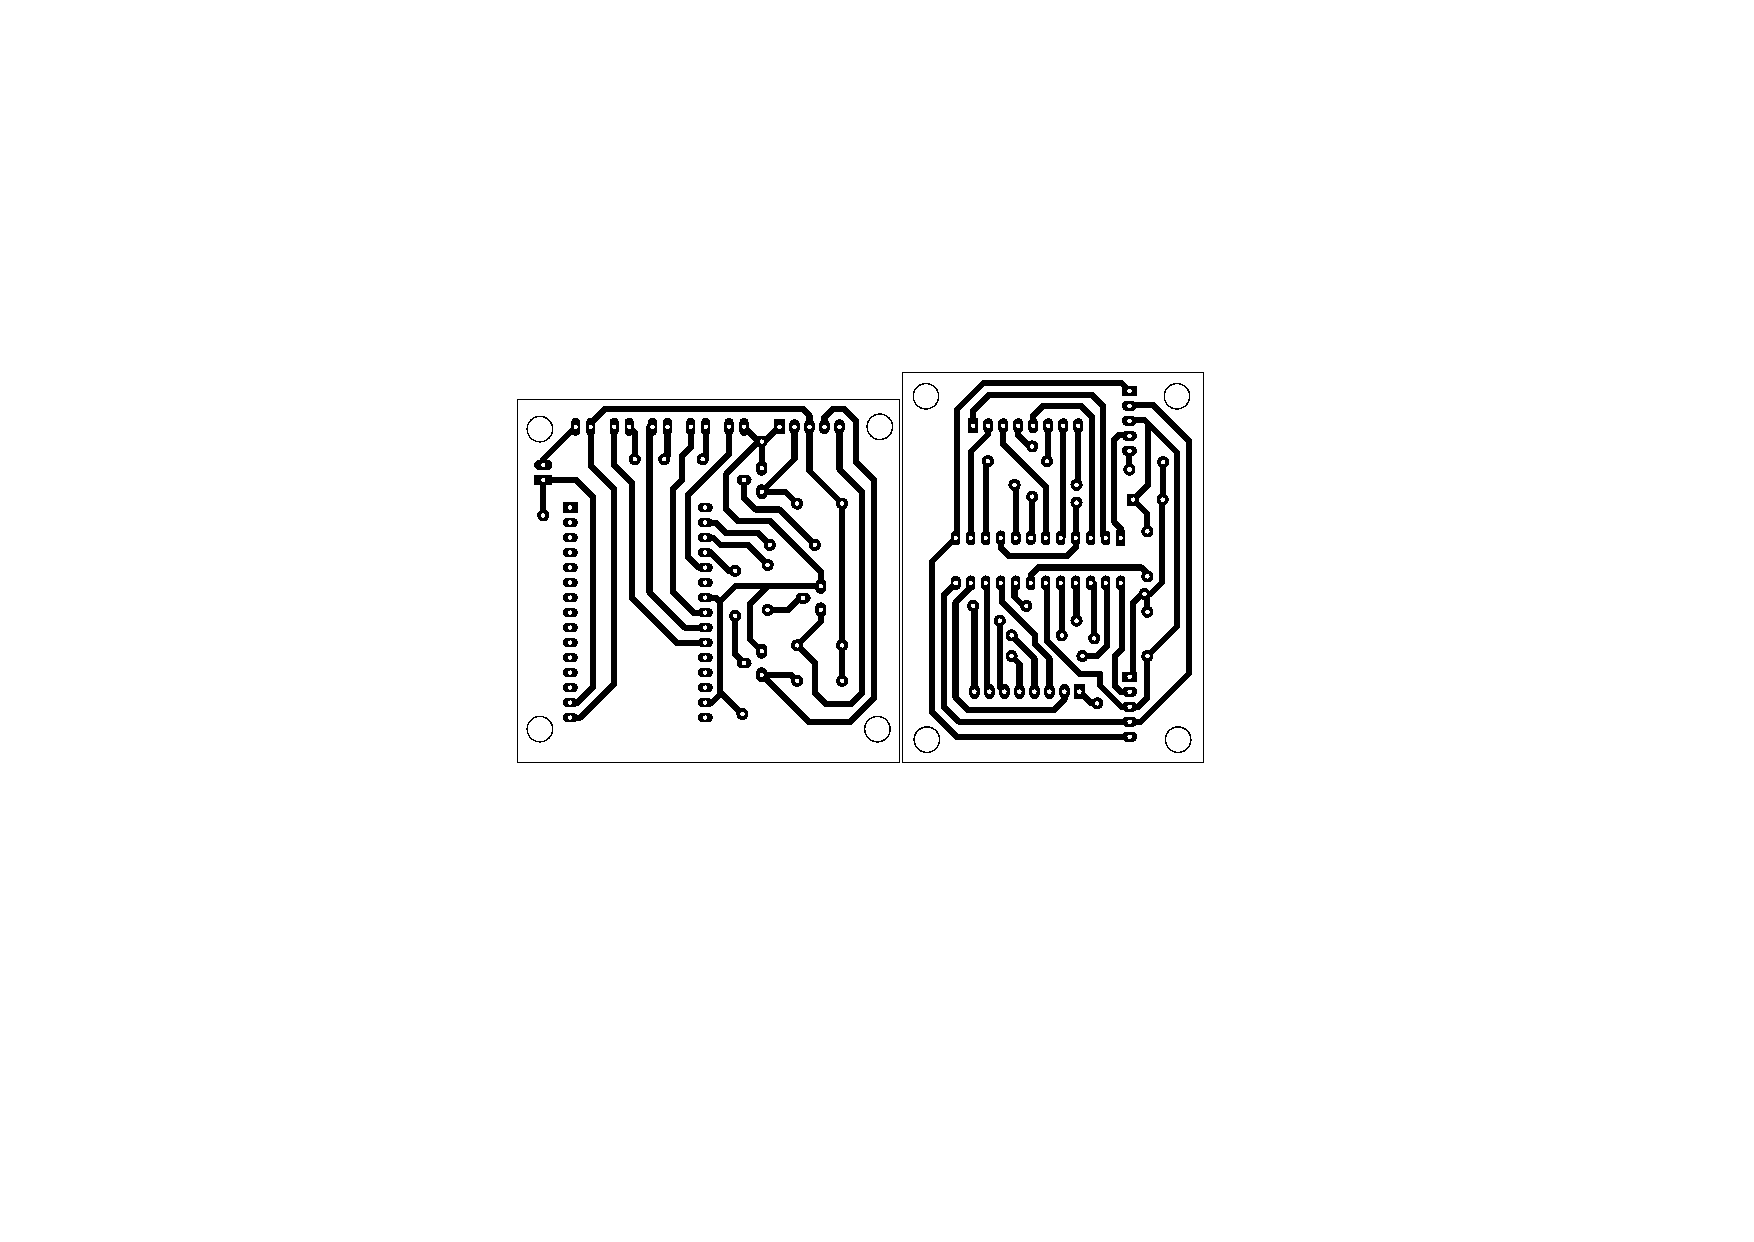
\includegraphics[width=\linewidth]{imagenes/hw/imp.pdf}
	\caption{Impresión PCB del módulo maestro y esclavo.}
	\label{fig:imp-pcb}
\end{figure}

\subsection{Presupuesto} \label{sec:presupuesto}

	Como se mencionó anteriormente, el cartel cuenta con un único módulo funcional maestro, y \texttt{N} módulos esclavos. Los precios están en pesos al momento de la ejecución de su respectiva compra. En el presupuesto no se tuvieron en cuenta los componentes e insumos varios (cables, gabinete, estaño, etc) ni los costos de las herramientas necesarias (soldador, multímetro, gafas de seguridad. etc.), ni el costo de impresión en el papel fotográfico para el PCB.

\begin{table}[ht]
	\centering
	\caption{Presupuesto módulo Maestro}
	\begin{spreadtab}{{tabular}{cccc}}
		@ Item							& @ Unidades& @ Precio unidad (\$)	& @ Subtotal (\$)\\ \hline
		@ NodeMCU Esp8266				& 1			& :={200}				& b2*c2		\\
		@ PCB							& 1			& :={100}				& b3*c3		\\
		@ Transistor NPN\footnotemark	& 3	& :={4}	& b4*c4		\\
		@ Resistencia 56KOhm			& 3			& :={1}					& b5*c5		\\
		@ Resistencia 680Ohm			& 3			& :={1}					& b6*c6		\\
		@ Jumpers						& 4			& :={1}					& b7*c7		\\
		@ Jack con bornera				& 1			& :={20}				& b8*c8		\\
		@ Pulsador						& 1			& :={20}				& b9*c9		\\
		@ Tecla Rocker Switch 			& 1			& :={30}				& b10*c10	\\
		@ Regleta de 1x15 pines hembra	& 2			& :={7}					& b11*c11	\\
		@ Hoja A4 fotográfico			& 1			& :={20}				& b12*c12	\\\hline
		@ Total							& 			&						& \$ :={sum(d2:d12)}\\ \hline
	\end{spreadtab}
\end{table}

\footnotetext{Del tipo 2n2222 o similar, para el testeo se utilizó el transistor 2n2369.}

\begin{table}[ht]
	\centering
	\caption{Presupuesto módulo Esclavo}
	\begin{spreadtab}{{tabular}{cccc}}
		@ Item									& @ Unidades& @ Precio unidad (\$)	& @ Subtotal (\$)\\ \hline
		@ LED									& 64		& :={1}					& b2*c2		\\
		@ PCB									& 1			& :={100}				& b3*c3		\\
		@ MAX7219								& 1			& :={45}				& b4*c4		\\
		@ Capacitor Polarizado	10µF			& 1			& :={3}					& b5*c5		\\
		@ Capacitor no polarizado 0.1µF			& 1			& :={3}					& b6*c6		\\
		@ Resistencia 24KOhm					& 1			& :={1}					& b7*c7		\\
		@ Conector hembra 8 Pin	(25.4mm)		& 2			& :={15}				& b8*c8		\\
		@ Conector hembra 5 Pin	(25.4mm)		& 2			& :={10}				& b9*c9		\\
		@ Regleta de 1x12 pines hembra (1.27mm)	& 2			& :={7}					& b10*c10	\\
		@ Hoja A4 fotográfico					& 1			& :={20}				& b11*c11	\\\hline
		@ Total									& 			&						& \$ :={sum(d2:d11)}\\ \hline
	\end{spreadtab}
\end{table}
